\documentclass[a4paper, 15pt, oneside]{book}
\usepackage[utf8]{inputenc}
\usepackage[margin=3cm, bindingoffset=1cm]{geometry}
\linespread{1.5}
\usepackage[backend=biber, sorting=none]{biblatex}
\addbibresource{bib.bib}
\usepackage{float}
\usepackage{csquotes}
\usepackage{subfig}
\usepackage{graphicx}
\usepackage{indentfirst}
\usepackage{fancyhdr}
\usepackage{geometry}
\usepackage{array}
\usepackage[hidelinks]{hyperref}
\setlength{\parindent}{1cm}
\usepackage{tcolorbox}


%\usepackage[Lenny]{fncychap}

\pagestyle{fancy}
\renewcommand{\chaptermark}[1]{\markboth{\thechapter.\ \uppercase{#1}}{}}
\fancyhf{}
\fancyhead[C]{\textbf{\leftmark}}
\fancyfoot[C]{\thepage}
\renewcommand{\headrulewidth}{1pt}
\renewcommand{\footrulewidth}{1pt}
\usepackage[Conny]{fncychap}

\title{Embedded System Project}
\author{Group 7}
\date{May 2024}

\renewcommand{\contentsname}{\bf Indice}
\renewcommand{\chaptername}{Capitolo}

\newenvironment{dedication}
  {\clearpage           % we want a new page
   \thispagestyle{empty}% no header and footer
   \vspace*{\stretch{1}}% some space at the top 
   \itshape             % the text is in italics
   \raggedleft          % flush to the right margin
  }
  {\par % end the paragraph
   \vspace{\stretch{3}} % space at bottom is three times that at the top
   \clearpage           % finish off the page
  }
  
\begin{document}
%Frontespizio
\begin{titlepage}
    \begin{center}
        \LARGE{\uppercase{Università degli Studi di Salerno}}\\
        \vspace{5mm}
        %Dipartimento
    	\uppercase{\normalsize \textbf{Dipartimento di Ingegneria dell'Informazione ed Elettrica e Matematica Applicata} }\\
    \end{center}
    \begin{figure}[H]
        \centering
        
\includegraphics[width=0.35\textwidth]{logo_unisa}
    \end{figure}
    
    \begin{center}
        %Corso di Laurea
    	\normalsize{ Corso di Laurea Magistrale in Ingegneria Informatica }\\
    	\vspace{15mm}
    	%Titolo
        {\LARGE{\bf \uppercase{Warpex}}}\\
    	\vspace{3mm}
    \end{center}
    
    \vspace{15mm}
    \noindent

\begin{center}
\begin{tabular}{ | c | c | c | c |} \hline
    \textbf{Nome} & \textbf{Cognome} & \textbf{Matricola} & \textbf{E-Mail} \\ \hline
        Michele & Martino & 0622702424 & m.martino48@studenti.unisa.it \\
        \hline
        Francesco & Quagliuolo & 0622702412 & f.quagliuolo@studenti.unisa.it \\
        \hline
        Emanuele & Relmi & 0622702368 & e.relmi@studenti.unisa.it \\
        \hline
        Benito & Senese & 0622702425 & b.senese1@studenti.unisa.it \\
        \hline
    \end{tabular}
\end{center}
    
    \vspace{20mm}
    
    %Anno Accademico
    \centering{\large \uppercase{ Anno Accademico 2023/2024 }}

\end{titlepage}


%Corpo della Tesi
\tableofcontents
\clearpage
\sloppy
\hyphenpenalty=10000
\exhyphenpenalty=10000

\chapter{\bf{User Stories}}

\section{US1 - Apertura Cancello}
\begin{tcolorbox}[title={Descrizione}, colback=red!20!white, colframe=red!80!black]
    \textbf{Come} utente, \\
    \textbf{voglio} premere il pulsante B1 quando il cancello è chiuso o in chiusura, \\
    \textbf{al fine di} avviare la fase di apertura del cancello.
\end{tcolorbox}

\begin{tcolorbox}[title={Criterio di Accettazione}, colback=blue!20!white, colframe=blue!80!black]
    \textbf{Dato che} il cancello è chiuso o in fase di chiusura, \\
    \textbf{quando} premo il pulsante B1, \\
    \textbf{allora} il cancello deve iniziare la fase di apertura.
\end{tcolorbox}

\section{US2 - Chiusura Cancello}
\begin{tcolorbox}[title={Descrizione}, colback=red!20!white, colframe=red!80!black]
    \textbf{Come} utente, \\
    \textbf{voglio} premere il pulsante B1 quando il cancello è in apertura o aperto, \\
    \textbf{al fine di} avviare la fase di chiusura del cancello.
\end{tcolorbox}

\begin{tcolorbox}[title={Criterio di Accettazione}, colback=blue!20!white, colframe=blue!80!black]
    \textbf{Dato che} il cancello è aperto o in fase di apertura, \\
    \textbf{quando} premo il pulsante B1, \\
    \textbf{allora} il cancello deve iniziare la fase di chiusura.
\end{tcolorbox}

\section{US3 - Regolazione Tempo Chiusura Automatica}
\begin{tcolorbox}[title={Descrizione}, colback=red!20!white, colframe=red!80!black]
    \textbf{Come} utente, \\
    \textbf{voglio} regolare il tempo di chiusura automatica del cancello premendo il pulsante B2 quando il cancello è chiuso, \\
    \textbf{al fine di} impostare dopo quanto tempo dall’apertura il cancello deve richiudersi.
\end{tcolorbox}

\begin{tcolorbox}[title={Criterio di Accettazione \#1}, colback=blue!20!white, colframe=blue!80!black]
    \textbf{Dato che} il cancello è chiuso, \\
    \textbf{quando} premo il pulsante B2, \\
    \textbf{se} il tempo di chiusura automatica è inferiore a 120 secondi, \\
    \textbf{allora} il tempo di chiusura automatica aumenta di 10 secondi.
\end{tcolorbox}

\begin{tcolorbox}[title={Criterio di Accettazione \#2}, colback=blue!20!white, colframe=blue!80!black]
    \textbf{Dato che} il cancello è chiuso, \\
    \textbf{quando} premo il pulsante B2, \\
    \textbf{se} il tempo di chiusura automatica è a 120 secondi, \\
    \textbf{allora} il tempo di chiusura automatica ritorna a 10 secondi.
\end{tcolorbox}

\section{US4 - Regolazione Tempo Lavoro}
\begin{tcolorbox}[title={Descrizione}, colback=red!20!white, colframe=red!80!black]
    \textbf{Come} utente, \\
    \textbf{voglio} regolare la durata delle fasi di apertura e chiusura del cancello premendo il pulsante B3 quando il cancello è chiuso, \\
    \textbf{al fine di} impostare la durata delle fasi di apertura e chiusura del cancello.
\end{tcolorbox}

\begin{tcolorbox}[title={Criterio di Accettazione \#1}, colback=blue!20!white, colframe=blue!80!black]
    \textbf{Dato che} il cancello è chiuso, \\
    \textbf{quando} premo il pulsante B3, \\
    \textbf{se} il tempo di lavoro è inferiore a 120 secondi, \\
    \textbf{allora} il tempo di lavoro aumenta di 10 secondi.
\end{tcolorbox}

\begin{tcolorbox}[title={Criterio di Accettazione \#2}, colback=blue!20!white, colframe=blue!80!black]
    \textbf{Dato che} il cancello è chiuso, \\
    \textbf{quando} premo il pulsante B3, \\
    \textbf{se} il tempo di lavoro è 120 secondi, \\
    \textbf{allora} il tempo di lavoro ritorna a 10 secondi.
\end{tcolorbox}

\section{US5 - Riapertura Automatica con Rilevazione Ostacolo}
\begin{tcolorbox}[title={Descrizione}, colback=red!20!white, colframe=red!80!black]
    \textbf{Come} utente, \\
    \textbf{voglio} che il cancello si riapra automaticamente se viene rilevata la presenza di un ostacolo durante la fase di chiusura, \\
    \textbf{in modo da} evitare danni al cancello e garantire la sicurezza delle persone e degli oggetti presenti.
\end{tcolorbox}

\begin{tcolorbox}[title={Criterio di Accettazione}, colback=blue!20!white, colframe=blue!80!black]
    \textbf{Dato che} il cancello è in fase di chiusura, \\
    \textbf{quando} il sensore di presenza (P1) rileva un ostacolo, \\
    \textbf{allora} il cancello si riapre automaticamente.
\end{tcolorbox}

\section{US6 - Gestione Sicura del Cancello in Presenza di Ostacoli}
\begin{tcolorbox}[title={Descrizione}, colback=red!20!white, colframe=red!80!black]
    \textbf{Come} utente, \\
    \textbf{voglio} che il dispositivo ignori le richieste di apertura o chiusura del cancello quando il sensore di presenza è attivo, \\
    \textbf{in modo da} prevenire movimenti non sicuri del cancello in presenza di ostacoli o persone.
\end{tcolorbox}

\begin{tcolorbox}[title={Criterio di Accettazione \#1}, colback=blue!20!white, colframe=blue!80!black]
    \textbf{Dato che} il sensore di presenza (P1) è attivo, \\
    \textbf{quando} c'è una richiesta di apertura o chiusura del cancello, \\
    \textbf{allora} il dispositivo non esegue l'azione richiesta.
\end{tcolorbox}

\begin{tcolorbox}[title={Criterio di Accettazione \#2}, colback=blue!20!white, colframe=blue!80!black]
    \textbf{Dato che} il sensore di presenza (P1), \\
    \textbf{quando} non rileva più alcun ostacolo, \\
    \textbf{allora} il dispositivo è nuovamente pronto a ricevere e gestire le richieste di apertura o chiusura del cancello..
\end{tcolorbox}

\section{US7 - Gestione del sensore di chiusura per determinare lo stato del cancello}
\begin{tcolorbox}[title={Descrizione}, colback=red!20!white, colframe=red!80!black]
    \textbf{Come} utente, \\
    \textbf{voglio} che il dispositivo utilizzi il sensore di presenza (P2) come sensore di chiusura del cancello\\
    \textbf{in modo da} determinare in modo affidabile lo stato del cancello.
\end{tcolorbox}

\begin{tcolorbox}[title={Criterio di Accettazione}, colback=blue!20!white, colframe=blue!80!black]
    \textbf{Dato che} il cancello è chiuso, \\
    \textbf{quando} il sensore di presenza (P2) è attivo, \\
    \textbf{allora} il cancello si considera chiuso.
\end{tcolorbox}

\section{US8 - Errore in caso di malfunzionamento del sensore di chiusura}
\begin{tcolorbox}[title={Descrizione}, colback=red!20!white, colframe=red!80!black]
    \textbf{Come} utente\\
    \textbf{voglio} che il dispositivo entri in uno stato di errore se il sensore di chiusura (P2) non si attiva dopo il tempo di lavoro previsto durante la fase di chiusura del cancello,\\
    \textbf{in modo da} essere avvisato in caso di malfunzionamento del sensore.
\end{tcolorbox}

\begin{tcolorbox}[title={Criterio di Accettazione}, colback=blue!20!white, colframe=blue!80!black]
    \textbf{Dato che} è in corso la fase di chiusura del cancello, \\
    \textbf{quando} il sensore di chiusura (P2) non si attiva entro il tempo di lavoro previsto, \\
    \textbf{allora} il dispositivo entra in uno stato di errore.
\end{tcolorbox}

\section{US9 - Avvio Chiusura Cancello senza Sensore Attivo}
\begin{tcolorbox}[title={Descrizione}, colback=red!20!white, colframe=red!80!black]
    \textbf{Come} utente, \\
    \textbf{voglio} che il dispositivo avvii la procedura di chiusura del cancello quando viene acceso, se il sensore di chiusura (P2) e il sensore di presenza (P1) non sono attivi, \\
    \textbf{in modo da} garantire la chiusura corretta del cancello all'accensione.
\end{tcolorbox}

\begin{tcolorbox}[title={Criterio di Accettazione}, colback=blue!20!white, colframe=blue!80!black]
    \textbf{Dato che} il dispositivo è acceso, \\
    \textbf{quando} il sensore di chiusura (P2) e il sensore di presenza (P1) non sono attivi, \\
    \textbf{allora} viene avviata la procedura di chiusura del cancello.
\end{tcolorbox}

\section{US10 - Indicazione del Cancello in Movimento}
\begin{tcolorbox}[title={Descrizione}, colback=red!20!white, colframe=red!80!black]
    \textbf{Come} utente, \\
    \textbf{voglio} che il LED giallo lampeggi mentre il cancello è in apertura o in chiusura, \\
    \textbf{al fine di} avere una conferma visiva dello stato di movimento.
\end{tcolorbox}

\begin{tcolorbox}[title={Criterio di Accettazione}, colback=blue!20!white, colframe=blue!80!black]
    \textbf{Dato} che il cancello è in fase di apertura o chiusura, \\
    \textbf{quando} il cancello si muove, \\
    \textbf{allora} il LED giallo lampeggia con una frequenza di 0,5 Hz.
\end{tcolorbox}

\section{US11 - Indicazione di Errore di Chiusura}
    \begin{tcolorbox}[title={Descrizione}, colback=red!20!white, colframe=red!80!black]
    \textbf{Come} utente, \\
    \textbf{voglio} che il LED rosso si accenda se il cancello non si chiude entro 10 secondi dal completamento del tempo di lavoro, \\
    \textbf{al fine di} essere notificato di uno stato di errore.
\end{tcolorbox}

\begin{tcolorbox}[title={Criterio di Accettazione}, colback=blue!20!white, colframe=blue!80!black]
    \textbf{Dato} che il cancello è in fase di chiusura, \\
    \textbf{quando} il cancello non si chiude entro 10 secondi dal completamento del tempo di lavoro, \\
    \textbf{allora} il LED rosso si accende per notificare lo stato di errore.
\end{tcolorbox}

\section{US12 - Indicazione di Ostacolo}
\begin{tcolorbox}[title={Descrizione}, colback=red!20!white, colframe=red!80!black]
    \textbf{Come} utente, \\
    \textbf{voglio} che il LED verde lampeggi se un ostacolo è presente davanti al sensore P1 quando si richiede l'apertura o la chiusura, \\
    \textbf{al fine di} essere notificato della presenza di un ostacolo.
\end{tcolorbox}

\begin{tcolorbox}[title={Criterio di Accettazione}, colback=blue!20!white, colframe=blue!80!black]
    \textbf{Dato} che il cancello è completamente aperto o chiuso, \\
    \textbf{quando} un ostacolo è presente davanti al sensore P1 e si richiede l'apertura o la chiusura del cancello, \\
    \textbf{allora} il LED verde lampeggia con una frequenza di 1 Hz per 30 secondi.
\end{tcolorbox}

\section{US13 - Indicazione Cancello Chiuso}
\begin{tcolorbox}[title={Descrizione}, colback=red!20!white, colframe=red!80!black]
    \textbf{Come} utente, \\
    \textbf{voglio} che tutti i LED siano spenti quando il cancello è chiuso, \\
    \textbf{al fine di} avere una conferma visiva che il cancello è completamente chiuso.
\end{tcolorbox}

\begin{tcolorbox}[title={Criterio di Accettazione}, colback=blue!20!white, colframe=blue!80!black]
    \textbf{Dato} che la procedura di chiusura del cancello è attiva, \\
    \textbf{quando} il cancello è completamente chiuso, \\
    \textbf{allora} tutti i LED sono spenti.
\end{tcolorbox}

\section{US14 - Indicazione Cancello Aperto}
\begin{tcolorbox}[title={Descrizione}, colback=red!20!white, colframe=red!80!black]
    \textbf{Come} utente, \\
    \textbf{voglio} che tutti i LED siano accesi senza lampeggiare quando il cancello è aperto, \\
    \textbf{al fine di} avere una conferma visiva che il cancello è completamente aperto.
\end{tcolorbox}

\begin{tcolorbox}[title={Criterio di Accettazione}, colback=blue!20!white, colframe=blue!80!black]
    \textbf{Dato} che la procedura di apertura del cancello è attiva, \\
    \textbf{quando} il cancello è completamente aperto, \\
    \textbf{allora} tutti i LED sono accesi senza lampeggiare.
\end{tcolorbox}
\chapter{\bf{Use Cases}}
\noindent Per poter rappresentare le user stories sopra descritte, utilizziamo gli Use Case Diagrams, dei diagrammi che rappresentano le interazioni tra gli utenti e il sistema.
In questo scenario, l'attore principale è l'utente che  interagisce con il sistema del cancello automatico attraverso i pulsanti B1, B2 e B3.


\section{Apertura Cancello [US1-US10-US14]}
L'utente ha la possibilità, in prossimità del cancello, di richiederne l'apertura premendo il pulsante B1. Quando il sistema rileva che il pulsante B1 è stato premuto e il cancello è nelle condizioni specificate (chiuso o in chiusura), avvia il processo di apertura del cancello. Il dispositivo inoltre fornisce un feedback visivo data dall'attivazione di un segnale luminoso, dato dal lampeggiamento di un LED giallo con frequenza 0.5 Hz.
Il dispositivo, inoltre, permette di verificare la completa apertura del cancello tramite l'accensione di tutti i LED: giallo, rosso e verde (figura \ref{usecase1}).

\begin{figure}
    \centering
    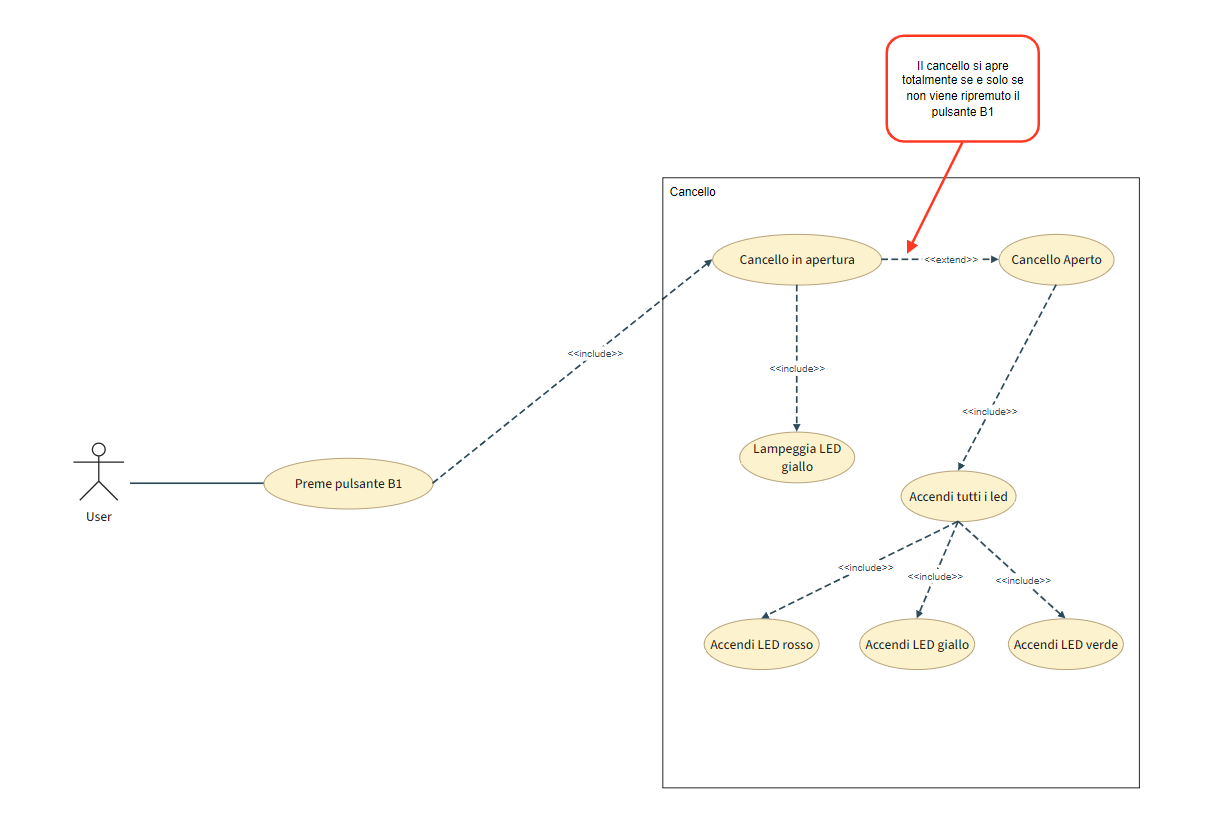
\includegraphics[width=0.9\textwidth]{figures/usecase_1.png}
    \caption{Apertura Cancello}
    \label{usecase1}
\end{figure}


\section{Chiusura Cancello [US2-US10-US13]}
L'utente ha la possibilità, in prossimità del cancello, di richiederne la chiusura premendo il pulsante B1. Quando il sistema rileva che il pulsante B1 è stato premuto e il cancello è nelle condizioni specificate (aperto o in apertura), avvia il processo di chiusura del cancello. Il dispositivo inoltre fornisce un feedback visivo data dall'attivazione di un segnale luminoso, dato dal lampeggiamento di un LED giallo con frequenza 0.5 Hz.
Il dispositivo, inoltre, permette di verificare la completa chiusura del cancello tramite lo spegnimento di tutti i LED (figura \ref{usecase2}).

\begin{figure}[H]
    \centering
    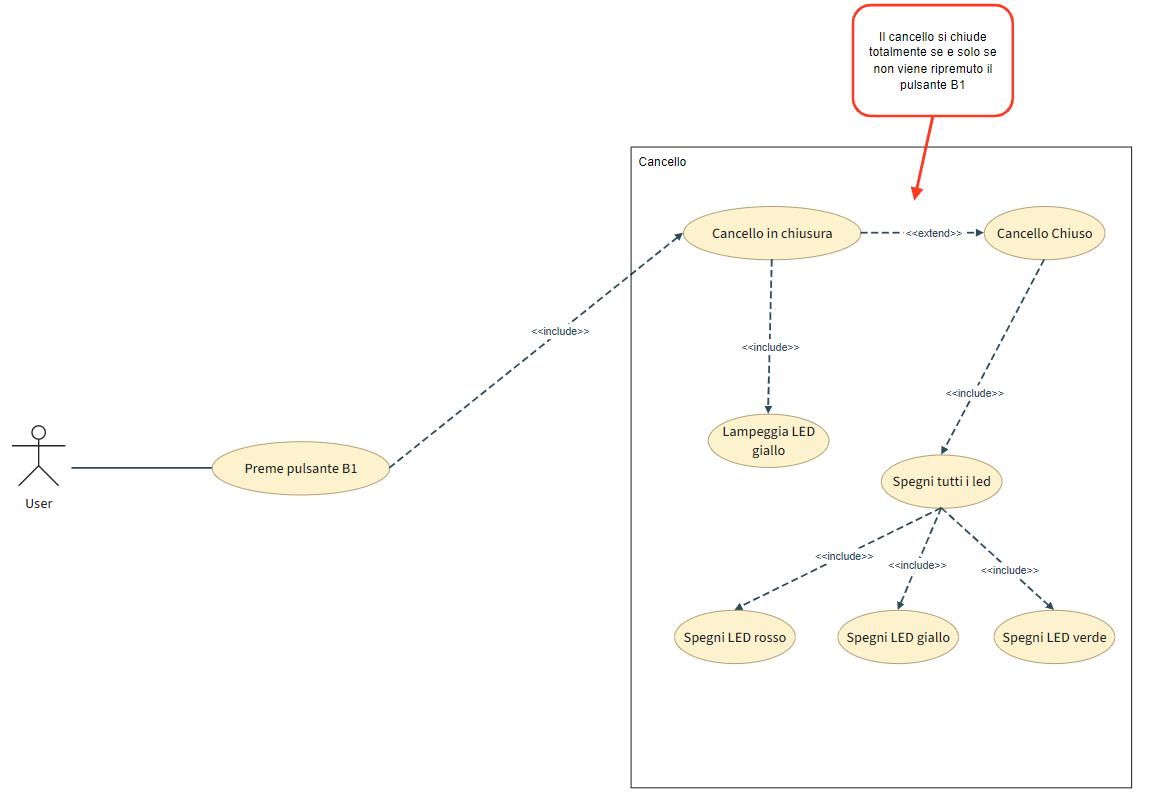
\includegraphics[width=0.9\textwidth]{figures/usecase_2.png}
    \caption{Chiusura Cancello}
    \label{usecase2}
\end{figure}


\section{Regolazione tempo di chiusura automatica [US3]}
L'utente ha la possibilità di regolare il tempo di chiusura automatica del cancello andando a determinare quanto esso debba rimanere aperto prima di chiudersi automaticamente.
Quando il cancello è chiuso, l'utente preme il pulsante B2 per effettuare la regolazione. Se il tempo di chiusura automatica è inferiore a 120 secondi, ogni pressione del pulsante B2 aumenta il tempo di 10 secondi. Se il tempo è già a 120 secondi, premendo nuovamente B2 il tempo viene riportato a 10 secondi (\ref{usecase3}).


\section{Regolazione Tempo di Lavoro [US4]}
L'utente ha la possibilità  di richiedere la regolazione della durata della fasi di apertura e chiusura del cancello premendo l'apposito pulsante (B3) solo quando il cancello è chiuso. Questa azione è essenziale per impostare la durata delle due fasi del cancello. Ogni pressione del pulsante incrementa la durata di 10 secondi e, se il tempo di lavoro è al suo massimo (120 secondi), esso ritorna a 10 secondi (\ref{usecase3}).

\begin{figure}[H]
    \centering
    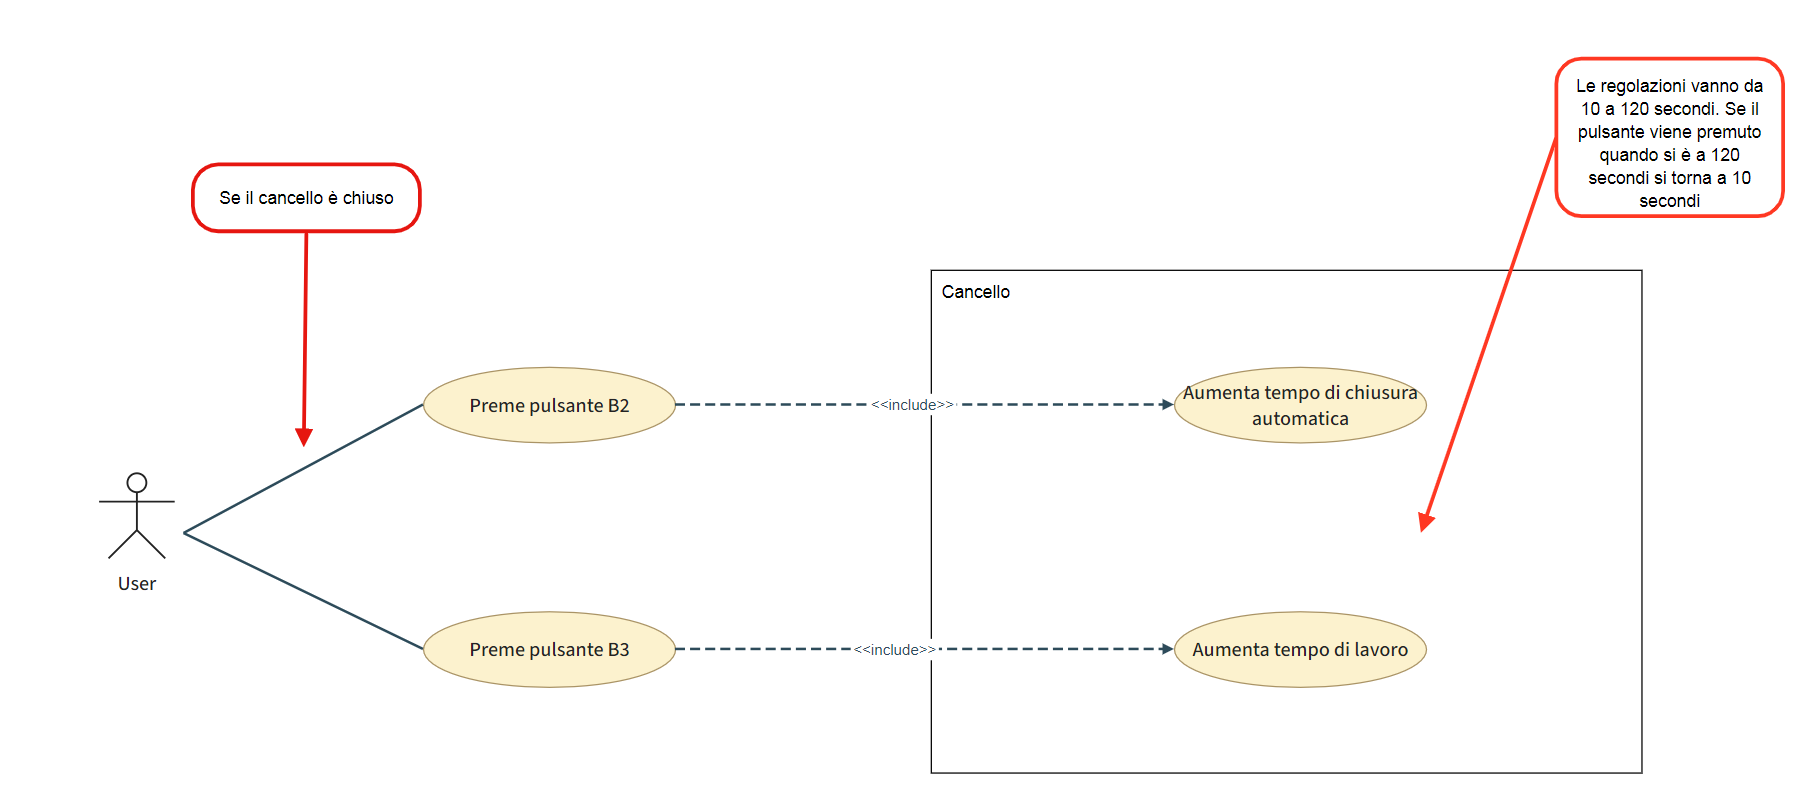
\includegraphics[width=0.9\textwidth]{figures/usecase_3.png}
    \caption{Regolazioni}
    \label{usecase3}
\end{figure}


\section{Riapertura Automatica con Rilevazione Ostacolo [US5-US14]}
L'utente ha la possibilità di richiedere la riapertura automatica del cancello se viene rilevata la presenza di un ostacolo durante la fase di chiusura tramite un sensore di presenza (P1). Questa azione è essenziale per evitare danni al cancello e garantire la sicurezza delle persone e degli oggetti presenti. 
Il dispositivo fornisce un feedback in caso di apertura completa del cancello, dato dall'accensione di tutti i LED (\ref{usecase5}).


\section{Gestione Richieste in presenza di ostacoli [US6-US12]}
L'utente ha la possibilità di richiedere che il dispositivo ignori le richieste di apertura o chiusura del cancello quando il sensore di presenza P1 è attivo. Questa azione è essenziale per prevenire movimenti non sicuri del cancello in presenza di ostacoli o persone.
Il dispositivo fornisce un feedback visivo in caso di presenza di un ostacolo, dato dal lampeggio del LED verde con frequenza di 1 Hz per un tempo di 30 secondi (\ref{usecase5}).


\begin{figure}[H]
    \centering
    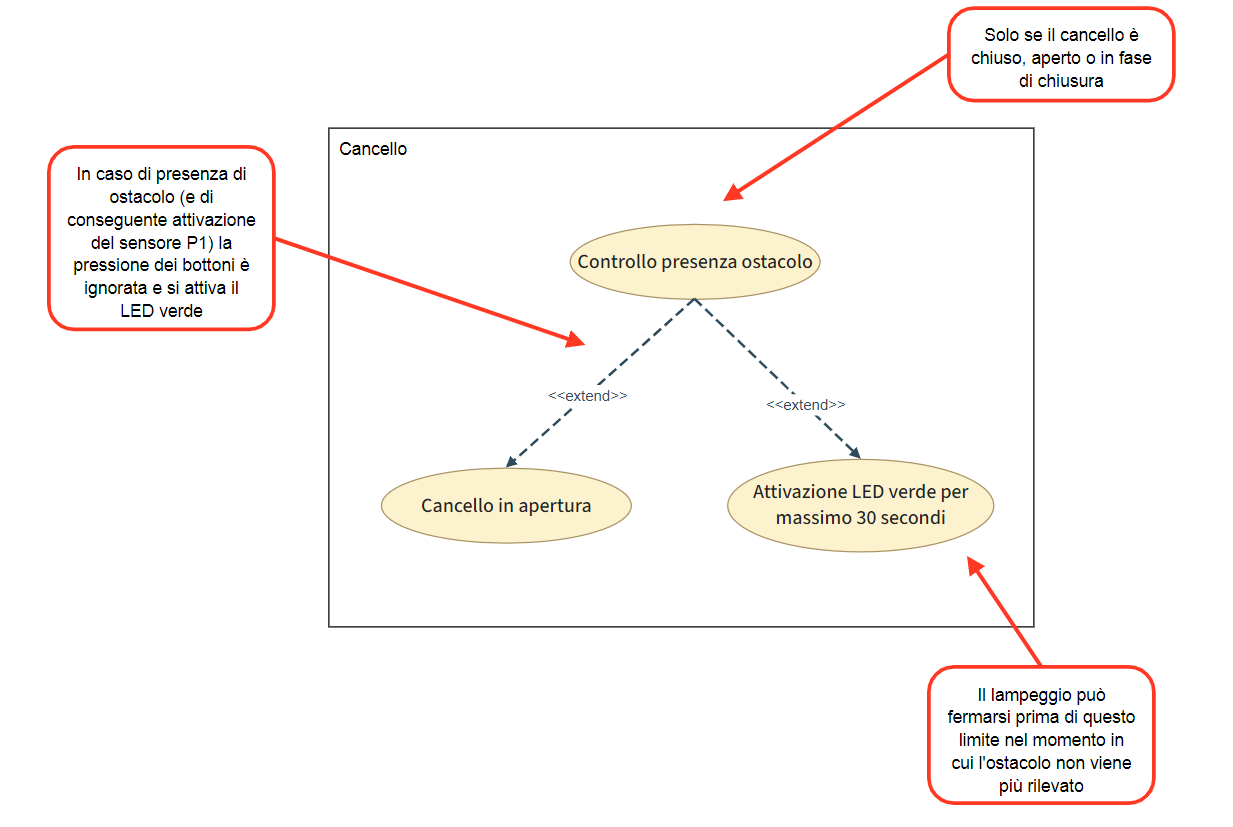
\includegraphics[width=0.9\textwidth]{figures/usecase_5.png}
    \caption{Controllo Ostacolo e Gestione Richieste}
    \label{usecase5}
\end{figure}


\section{Determinazione e Comunicazione stato cancello [US7-US13]}
L'utente ha la possibilità di richiedere la determinazione dello stato del cancello tramite un sensore di presenza (P2). Questa azione è essenziale per determinare correttamente lo stato del cancello che si considera chiuso quando il sensore è attivo (\ref{usecase7}). 
Il dispositivo fornisce un feedback visivo in caso il cancello risulti completamente chiuso, dato dallo spegnimento di tutti i LED.

\begin{figure}[H]
    \centering
    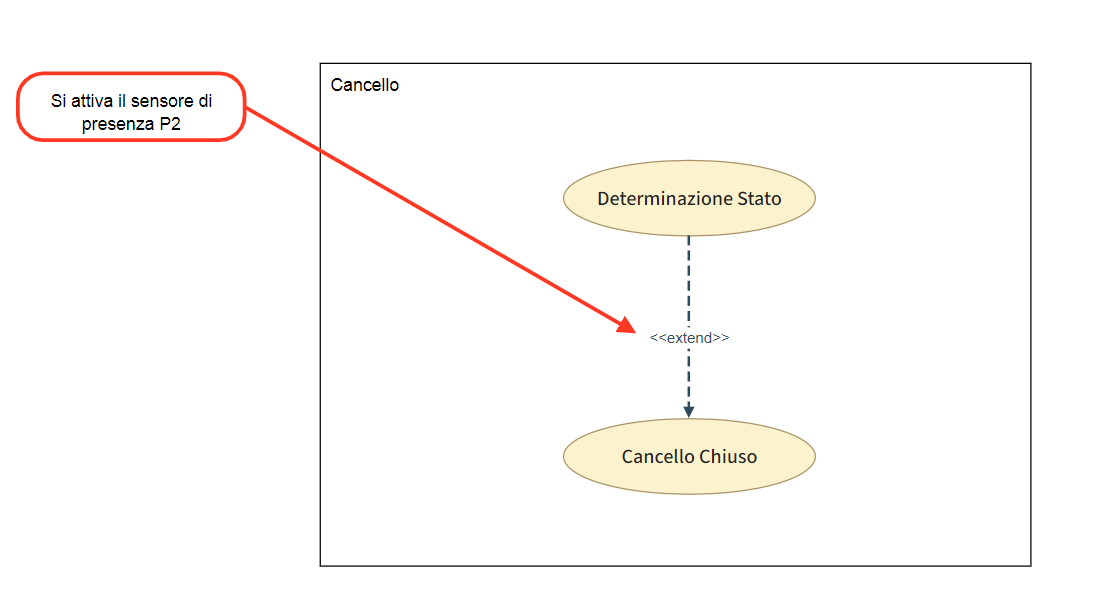
\includegraphics[width=0.9\textwidth]{figures/usecase_7.png}
    \caption{Determinazione Stato}
    \label{usecase7}
\end{figure}


\section{Gestione dello stato di errore [US8-US11]}
L'utente ha la possibilità di richiedere che il dispositivo entri in uno stato di errore nel caso in cui il sensore di presenza P2 non si attivi dopo il tempo di lavoro previsto durante la fase di chiusura del cancello. Questa azione è essenziale per far si che l'utente venga avvisato in caso di malfunzionamento del sensore.
Il dispositivo fornisce un feedback visivo dello stato di errore, dato dall'accensione del LED rosso in caso il cancello non si chiuda entro 10 secondi dal completamento del tempo di lavoro (\ref{usecase8}).

\begin{figure}[H]
    \centering
    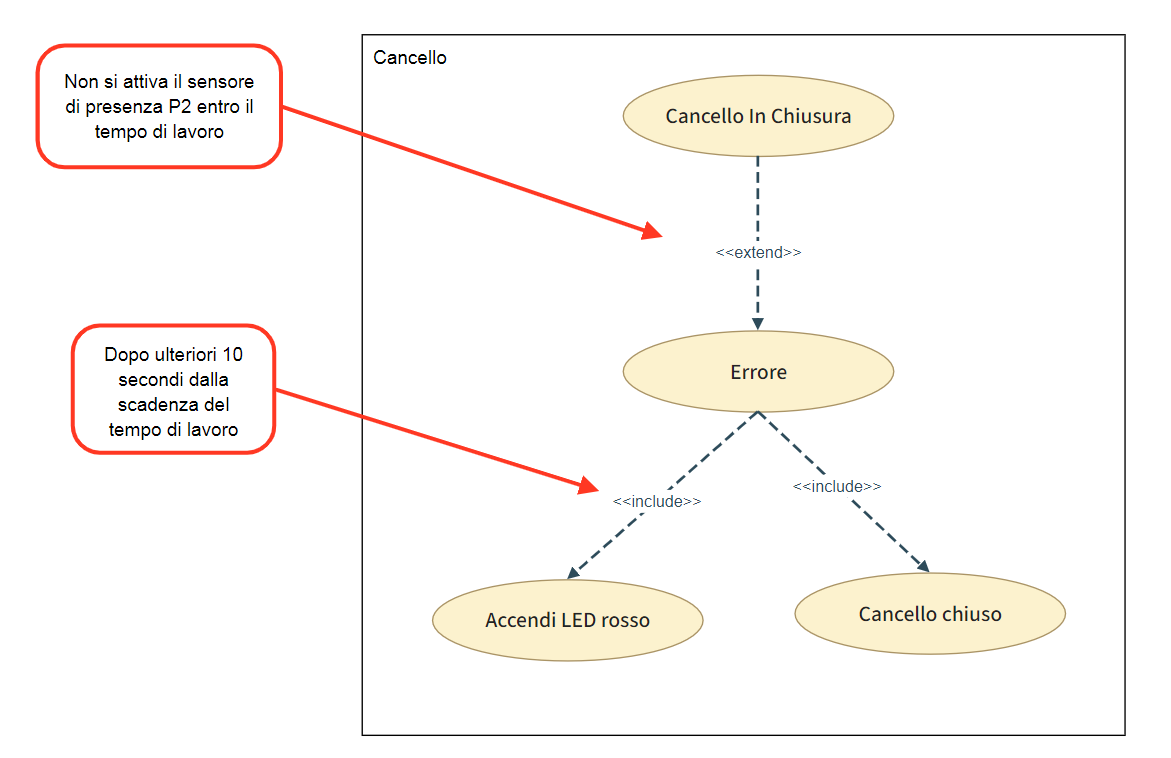
\includegraphics[width=0.9\textwidth]{figures/usecase_8.png}
    \caption{Stato di Errore}
    \label{usecase8}
\end{figure}


\section{Chiusura automatica all'accensione [US9]}
L'utente ha la possibilità di richiedere che il dispositivo avvii la procedura di chiusura del cancello automatico quando il dispositivo viene acceso per la prima volta, solo se i due sensori di presenza P1 e P2 non sono attivi. Questa azione è essenziale per garantire la corretta chiusura del cancello all'accensione del dispositivo.


\begin{figure}[H]
    \centering
    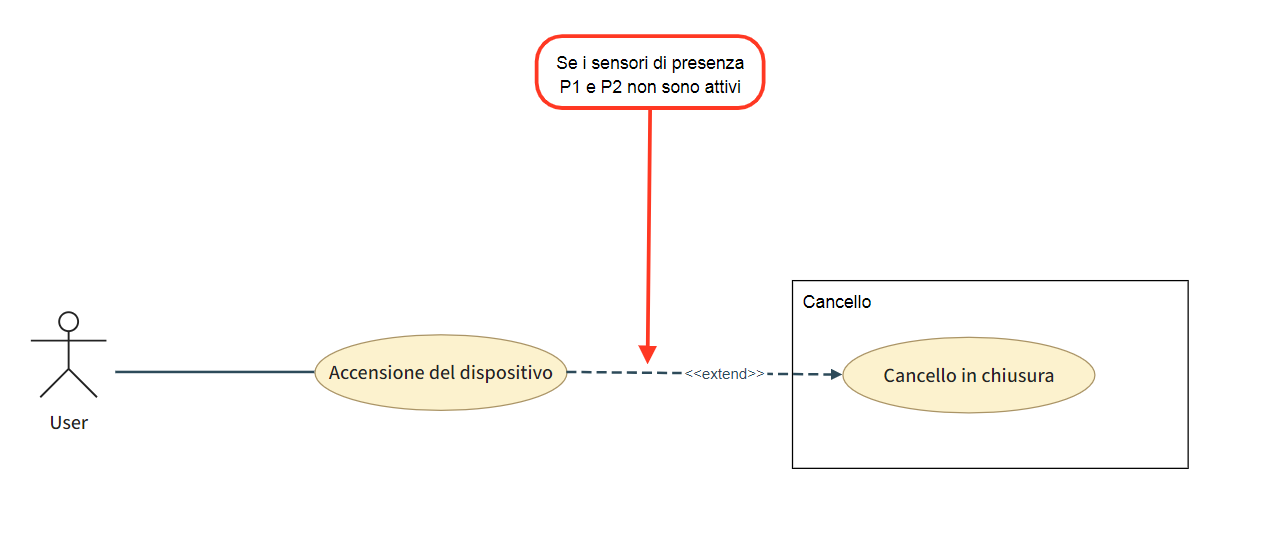
\includegraphics[width=0.9\textwidth]{figures/usecase_9.png}
    \caption{Chiusura Automatica}
    \label{usecase9}
\end{figure}


\section{General Use Case}
\begin{figure}[H]
    \centering
    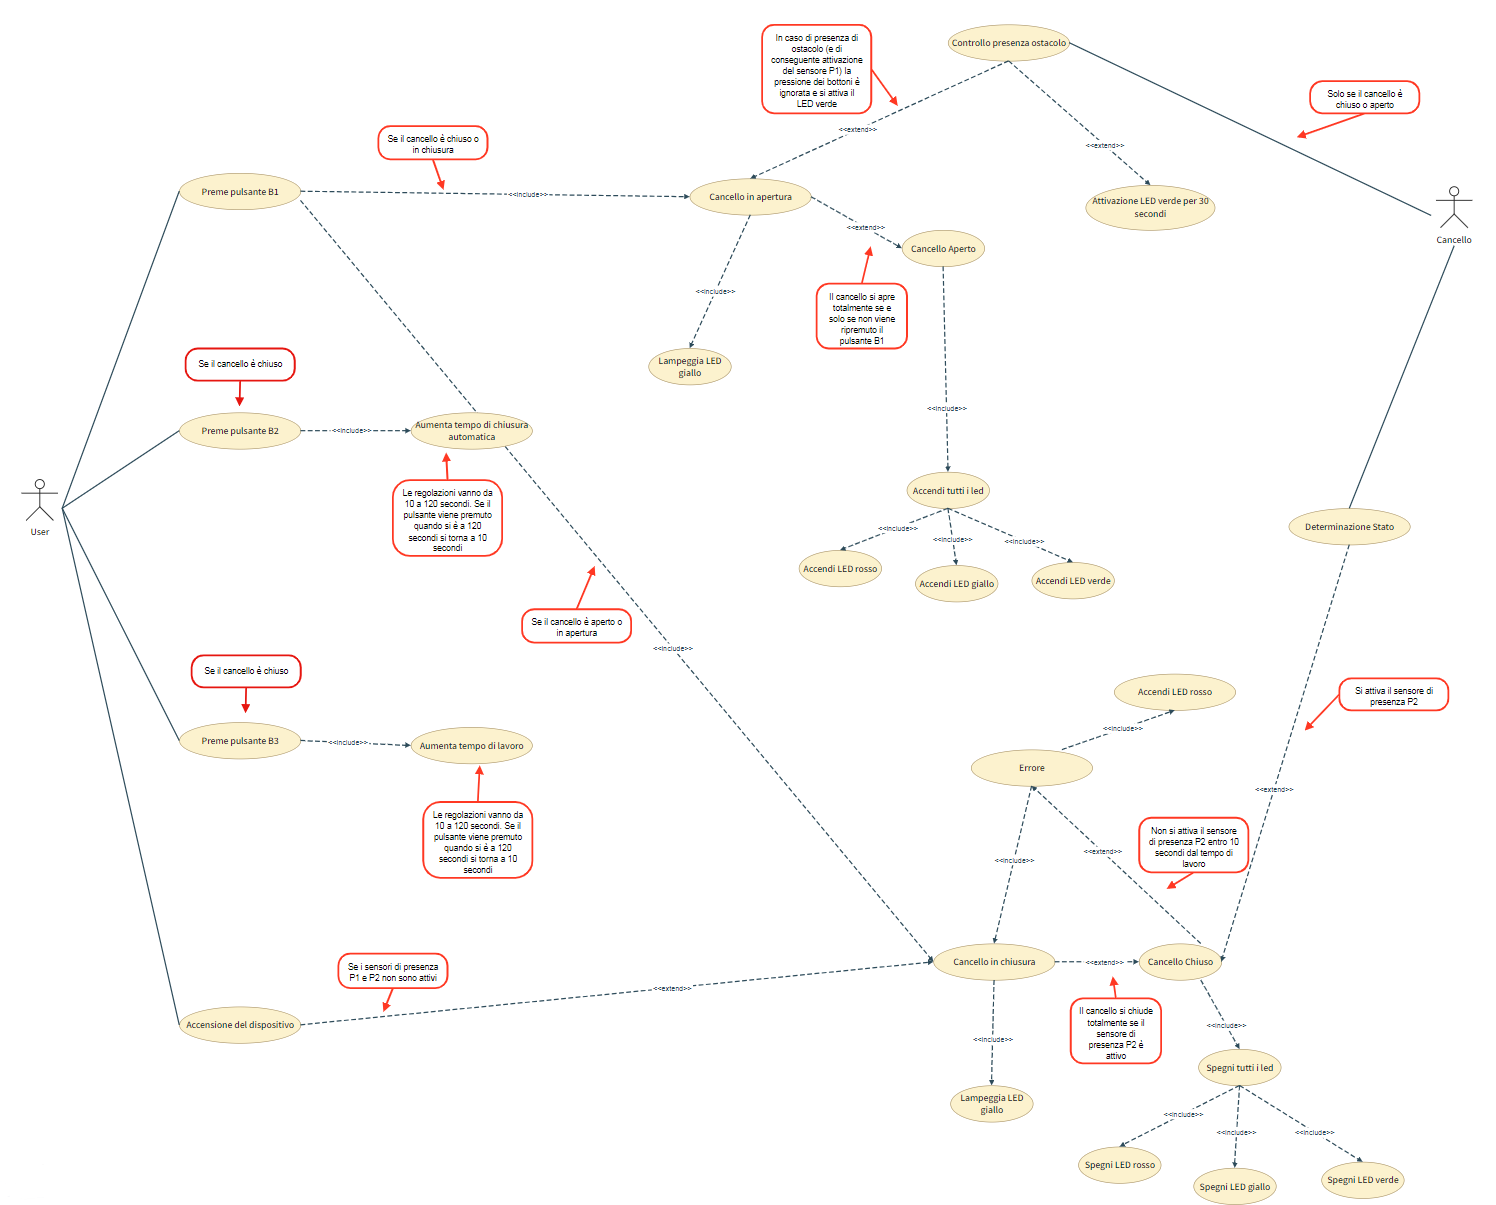
\includegraphics[width=1\linewidth]{figures/generalusecases.png}
    \caption{Use Cases Generale}
    \label{general}
\end{figure}
\chapter{\bf{Activity Diagrams}}

\section{Apertura e Chiusura Cancello   [Scenario 1]}
Questo scenario, presentato in figura \ref{scenario1}, descrive passo dopo passo le azioni che l’utente compie per aprire e chiudere il cancello, dalle fasi iniziali di richiesta tramite il pulsante B1, fino al feedback visivo che conferma l'operazione completata. Nel seguito verrà presentato il flusso di azioni associato allo scenario corrente:

\noindent Apertura del cancello:
\begin{enumerate}
    \item L’utente decide di aprire il cancello e si avvicina ad esso.
    \item Per avviare il processo di apertura, l’utente preme il pulsante B1.
    \item Il sistema rileva che il pulsante B1 è stato premuto.
    \item Il sistema verifica che il cancello sia chiuso o in chiusura.
    \item Il sistema avvia il processo di apertura del cancello.
    \item Durante l'apertura, il dispositivo fornisce un feedback visivo attivando il lampeggiamento del LED giallo con frequenza 0.5 Hz.
    \item Una volta completata l'apertura, tutti i LED (giallo, rosso e verde) si accendono per indicare la completa apertura del cancello.
\end{enumerate}


\noindent Chiusura del cancello:
\begin{enumerate}
    \item L’utente decide di chiudere il cancello e si avvicina ad esso.
    \item Per avviare il processo di chiusura, l’utente preme il pulsante B1.
    \item Il sistema rileva che il pulsante B1 è stato premuto.
    \item Il sistema verifica che il cancello sia aperto o in apertura.
    \item Il sistema avvia il processo di chiusura del cancello.
    \item Durante la chiusura, il dispositivo fornisce un feedback visivo attivando il lampeggiamento del LED giallo con frequenza 0.5 Hz.
    \item Una volta completata la chiusura, tutti i LED (giallo, rosso e verde) si spengono per indicare la completa chiusura del cancello.
\end{enumerate}


\begin{figure}[H]
    \centering
    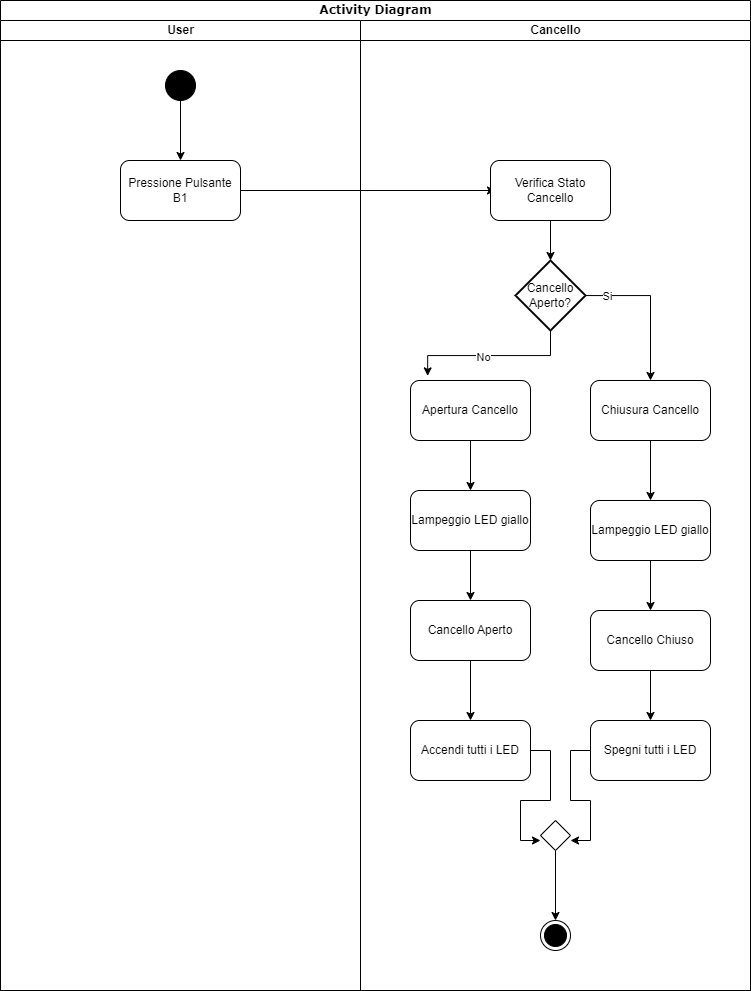
\includegraphics[width=0.9\textwidth]{figures/scenario1.drawio.png}
    \caption{Scenario 1}
    \label{scenario1}
\end{figure}


\section{Regolazioni [Scenario 2]}
Questo scenario, presentato in figura \ref{scenario2}, descrive passo dopo passo le azioni che l’utente compie per regolare il tempo di chiusura automatica del cancello. Nel seguito verrà presentato il flusso di azioni associato allo scenario corrente:

\noindent Regolazione tempo di chiusura automatica:

\begin{enumerate}
\item L’utente decide di regolare il tempo di chiusura automatica del cancello.
\item L’utente si avvicina al cancello chiuso.
\item Per avviare il processo di regolazione, l’utente preme il pulsante B2.
\item Il sistema rileva che il pulsante B2 è stato premuto.
\item Se il tempo di chiusura automatica è inferiore a 120 secondi, ogni pressione del pulsante B2 aumenta il tempo di 10 secondi.
\item Se il tempo di chiusura automatica è già a 120 secondi, premendo nuovamente B2 il tempo viene riportato a 10 secondi.
\end{enumerate}

Questo scenario descrive passo dopo passo le azioni che l’utente compie per regolare la durata delle fasi di apertura e chiusura del cancello. Per questioni di semplicità, il diagramma riguardante quest'attività non è stato riportato poiché identico al precedente.

\noindent Regolazione Tempo di Lavoro:

\begin{enumerate}
\item L’utente decide di regolare la durata delle fasi di apertura e chiusura del cancello.
\item L’utente si avvicina al cancello chiuso.
\item Per avviare il processo di regolazione, l’utente preme il pulsante B3.
\item Il sistema rileva che il pulsante B3 è stato premuto.
\item Ogni pressione del pulsante B3 incrementa la durata di 10 secondi.
\item Se il tempo di lavoro è al massimo (120 secondi), premendo nuovamente B3, il tempo viene riportato a 10 secondi.
\end{enumerate}


\begin{figure}[H]
    \centering
    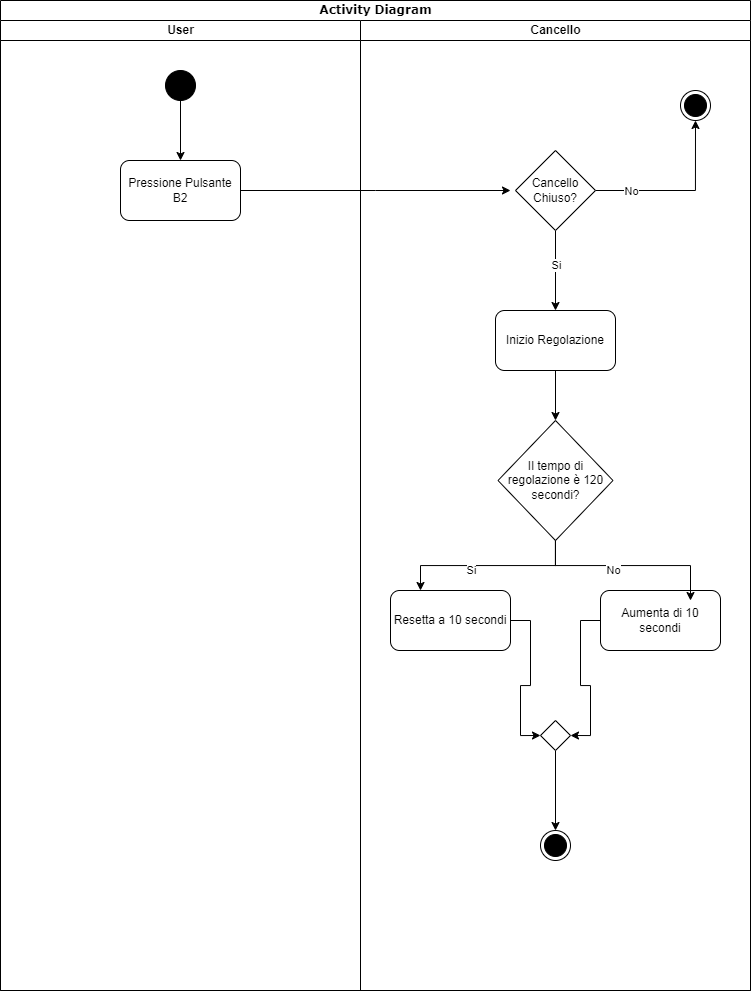
\includegraphics[width=0.9\textwidth]{figures/scenario2.drawio.png}
    \caption{Scenario 2}
    \label{scenario2}
\end{figure}


\section{Gestione Stato e Ostacoli [Scenario 3]}
Questo scenario, presentato in figura \ref{scenario3}, descrive passo dopo passo le azioni che l’utente compie per richiedere la riapertura automatica del cancello in presenza di un ostacolo. Nel seguito verrà presentato il flusso di azioni associato allo scenario corrente:

\noindent Riapertura Automatica con Rilevazione Ostacolo:

\begin{enumerate}
\item Il sistema rileva un ostacolo tramite il sensore di presenza (P1) durante la fase di chiusura del cancello.
\item Il sistema avvia la riapertura automatica del cancello per evitare danni e garantire la sicurezza.
\item Il dispositivo fornisce un feedback visivo in caso di apertura completa del cancello, accendendo tutti i LED (giallo, rosso e verde).
\item Se il sistema non rileva alcun ostacolo procederà con la chiusura del cancello e l'attivazione del sensore di presenza P2.
\end{enumerate}

\noindent Gestione Richieste in presenza di ostacoli:
Questo scenario descrive passo dopo passo le azioni che l’utente compie per gestire le richieste di apertura o chiusura del cancello in presenza di ostacoli. Nel seguito verrà presentato il flusso di azioni associato allo scenario corrente:


\begin{enumerate}
\item L’utente decide di attivare la funzione che fa ignorare le richieste di apertura o chiusura del cancello quando il sensore di presenza (P1) è attivo.
\item Il sistema rileva la presenza di un ostacolo tramite il sensore P1.
\item Il sistema ignora le richieste di apertura o chiusura del cancello per prevenire movimenti non sicuri.
\item Il dispositivo fornisce un feedback visivo della presenza di un ostacolo, facendo lampeggiare il LED verde con una frequenza di 1 Hz per 30 secondi.
\end{enumerate}


\begin{figure}[H]
    \centering
    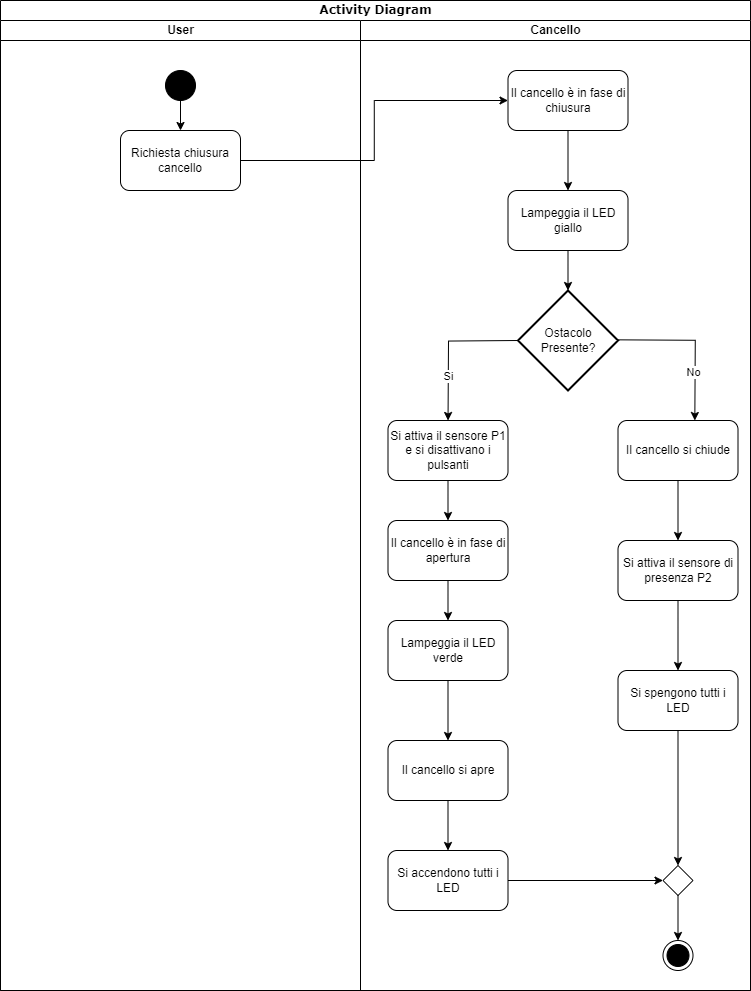
\includegraphics[width=0.9\textwidth]{figures/scenario3.drawio.png}
    \caption{Scenario 3}
    \label{scenario3}
\end{figure}


\section{Stato di Errore [Scenario 4]}
Questo scenario, presentato in figura \ref{scenario4}, descrive passo dopo passo le azioni che l’utente compie per far entrare il dispositivo in uno stato di errore in caso di malfunzionamento del sensore di presenza (P2). Nel seguito verrà presentato il flusso di azioni associato allo scenario corrente:

\noindent Stato di errore con rilevazione malfunzionamento del sensore:

\begin{enumerate}
\item L’utente richiede la chiusura del cancello tramite il pulsante B1
\item Il sistema rileva che il sensore di presenza (P2) non si è attivato dopo il tempo di lavoro previsto durante la fase di chiusura del cancello.
\item Il sistema entra in uno stato di errore per avvisare l’utente del possibile malfunzionamento del sensore.
\item Il dispositivo fornisce un feedback visivo dello stato di errore, accendendo il LED rosso se il cancello non si chiude entro 10 secondi dal completamento del tempo di lavoro.
\end{enumerate}

\begin{figure}[H]
    \centering
    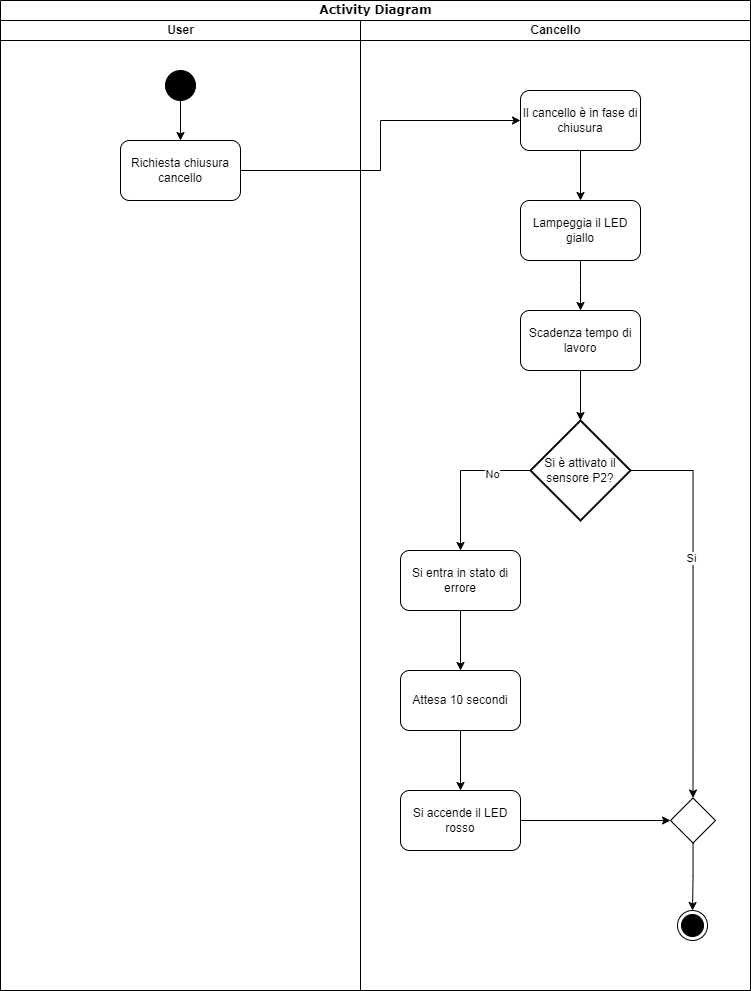
\includegraphics[width=0.9\textwidth]{figures/scenario4.drawio.png}
    \caption{Scenario 4}
    \label{scenario4}
\end{figure}


\section{Chiusura automatica all'accensione [Scenario 5]}
Questo scenario, presentato in Figura 2.7, descrive passo dopo passo le azioni che l’utente compie per richiedere la chiusura automatica del cancello all'accensione del dispositivo. Nel seguito verrà presentato il flusso di azioni associato allo scenario corrente:

\noindent Chiusura automatica all'accensione del dispositivo:

\begin{enumerate}
\item L’utente accende il dispositivo per la prima volta.
\item Il sistema verifica che i sensori di presenza P1 e P2 non siano attivi.
\item Il sistema avvia la procedura di chiusura del cancello.
\item Il dispositivo garantisce la corretta chiusura del cancello all'accensione.
\end{enumerate}


\begin{figure}[H]
    \centering
    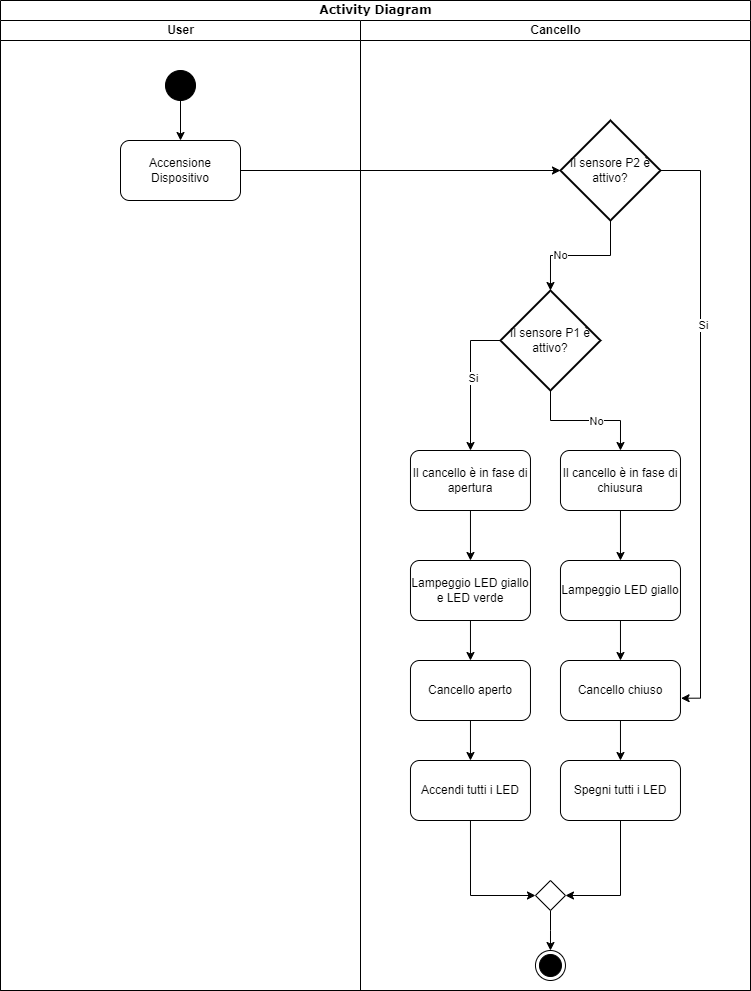
\includegraphics[width=0.9\textwidth]{figures/scenario5.drawio.png}
    \caption{Scenario 5}
    \label{scenario5}
\end{figure}
\chapter{\bf{State Diagrams}}
\clearpage
\phantomsection
\addcontentsline{toc}{chapter}{Indice delle Figure}

\renewcommand{\listfigurename}{\bf Indice delle Figure}
\listoffigures


%\chapter*{Acknowledgements}
%\addcontentsline{toc}{chapter}{Acknowledgements}
\clearpage
%\printbibliography[
%heading=bibintoc,
%title={References}
%]
\clearpage
%\listoffigures
%\addcontentsline{toc}{chapter}{\listfigurename}
\clearpage
%\listoftables
%\addcontentsline{toc}{chapter}{\listtablename}
\clearpage
\end{document}